\chapter{State Estimation}\label{cha3}
In this chapter is first an introduction in the Kalman Filter and the modified version called Extendend Kalman Filter given. In a second step will the state estimation algorithm, developed during this thesis explained. This gives an overview over the whole code and describes how the parameters were set and how a sensor data outage is handled. Section \ref{state_estimation} and \ref{sensor_estimation} will focus on the two essential parts of the algorithm, how the states are estimated and how the measurements are estimated.
\section{Extended Kalman Filter}

\subsection*{Discrete Kalman Filter}
First a short introduction is given what the Kalman Filter means and the basic computational origins are mentioned.
\begin{quote}The Kalman filter is an extremely effective versatile procedure for combining noisy sensor outputs to estimate the state of a system with uncertain dynamics.\end{quote} […angu...] It was published in 1960 by R.E.Kalman. The Filter gained a strong impact in the area of autonomous or assisted navigation [..pap...]. 
Systems in which the filter is estimating the state $x \in R^{n}$ can be described by the following linear stochastic difference equation.
\begin{equation}
x_{k+1}=A_k*x_k+B_k*u_k+w
\label{eq1}
\end{equation} The next equation shows the relation between the state and the measurement $z \in R^{n}$.
\begin{equation} 
z_k=H_k*x_k+D_k*u_k+v
\label{eq2}
\end{equation}
Where the random variables $w$ and $v$ stand for the process and the measurement noise assumed to be independent, white and normal probability distributions.
\begin{quote}The $n\times n$ matrix A in equation \ref{eq1} relates the state at time step $k$ to the state at step $k+1$, in the absene of either a dirving function or process noise. The $n\times l$ matrix $B$ relates the control input $u \in R^{l}$ to the state $x$. The $m \times m$ matrix $H$ in the measurement equation \ref{eq2} relates to the state to the measurement $z_k$.\end{quote}[.pap.]
Mostly the noisy sensors are a GPS receiver and inertial navigation system or other sensors for example speed sensors. The states of a system are described by the position, velocity, attitude and attitude rate [.angu..].

\subsection*{Mathematical Background}\label{math_kalman}
In figure \ref{simple_schematic} the structure of the algorithm is sketched for e better understanding of the filter's mathematical background . 
\begin{figure}[h]
\begin{center}
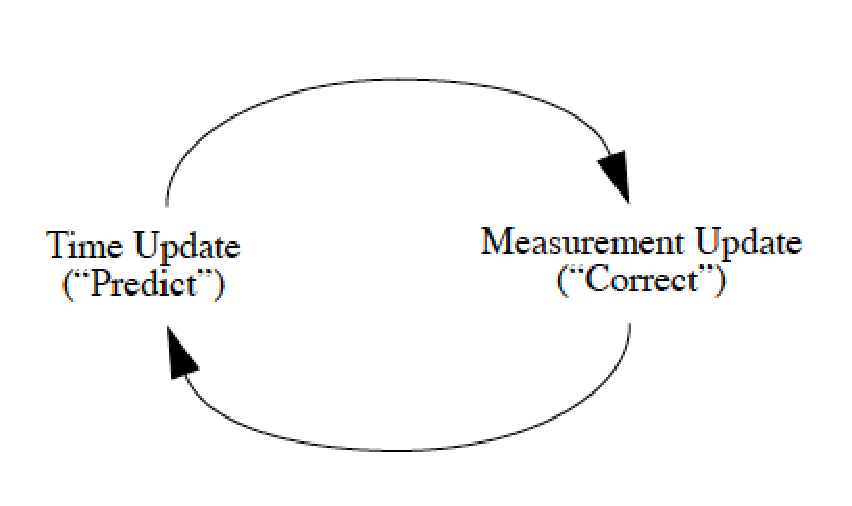
\includegraphics[width=6cm]{pictures/simple_schematic_algo.eps}
\caption{A simple structure of the algorithm}
\label{simple_schematic}
\end{center}
\end{figure}
In a first step the state at $k+1$ is estimated based on \ref{eq1}. This estimation is called a priori state estimation and written as $\hat{x}_k^{-}$. In a second step the a priori state estimation is corrected by the knowledge of measurements $z_k$. This corrected estimation is called the a posteriori estimation and written as $\hat{x}_k$.

Now two error can be defined with it's a error covariances. First the error of the a priori estimation 
\begin{equation}
e^{-}=x_k-\hat{x}_k^{-}
\end{equation}
and second the error of the a posteriori estimation 
\begin{equation}
e=x_k-\hat{x}_k
\end{equation}
with the a priori estimate error covariance 
\begin{equation}
P^{-}_k=E[e^{-}e^{-T}]
\end{equation}
and the a posteriori error covariance.
\begin{equation}
P_k=E[ee^{T}]\label{P_post}
\end{equation}

The Kalman Filter is calculating the a posteriori estimation, the one we are finally looking for. This calculation is a linear combination between the a priori estimated state and the difference of the the estimated measurement $x_k*H$ and the actual measurement $z_k$ weighted with the Kalman gain $K$. This difference $z_k-H_k\hat{x}^{-}_k$ is  called residual and tells us how accurate the estimation of the measurements is. In equation \ref{eq7} is this summerized.
\begin{equation}
\hat{x}_k^{-}*K*(z_k-H_k\hat{x}^{-}_k)\label{eq7}
\end{equation}
The Kalman gain $K$ is the heart of the Kalman Filter. $K$, a $n\times n$ Matrix is chosen in a way to minimize the a posteriori error covariance shown in equation \ref{P-post}. With some calculations the following 
\begin{equation}
K=\frac{P^{-}_k*H^{T}_k}{(H_k*P^{-}_k*H^{T}_k+R_k)}
\end{equation}
can be derived for the Kalman gain $K$.[..pap..]] 
This concept uses the information of a normal gaussian distribution of the noise mentioned in (..equ2..). $P_k$ is minimized using the Maximum Likelihood Estimation and is called the  Gaussian Maximum-Likelihood Estimator […]. A more detailed derivation of the mathematics is shown in [..maybeck..] and [..angu..].

\subsection*{Algorithm}
With equations described in the above section the estimation and correction step can be summarized as in figure \ref{equation_kalman} is shown.
\begin{figure}[h]
\begin{center}
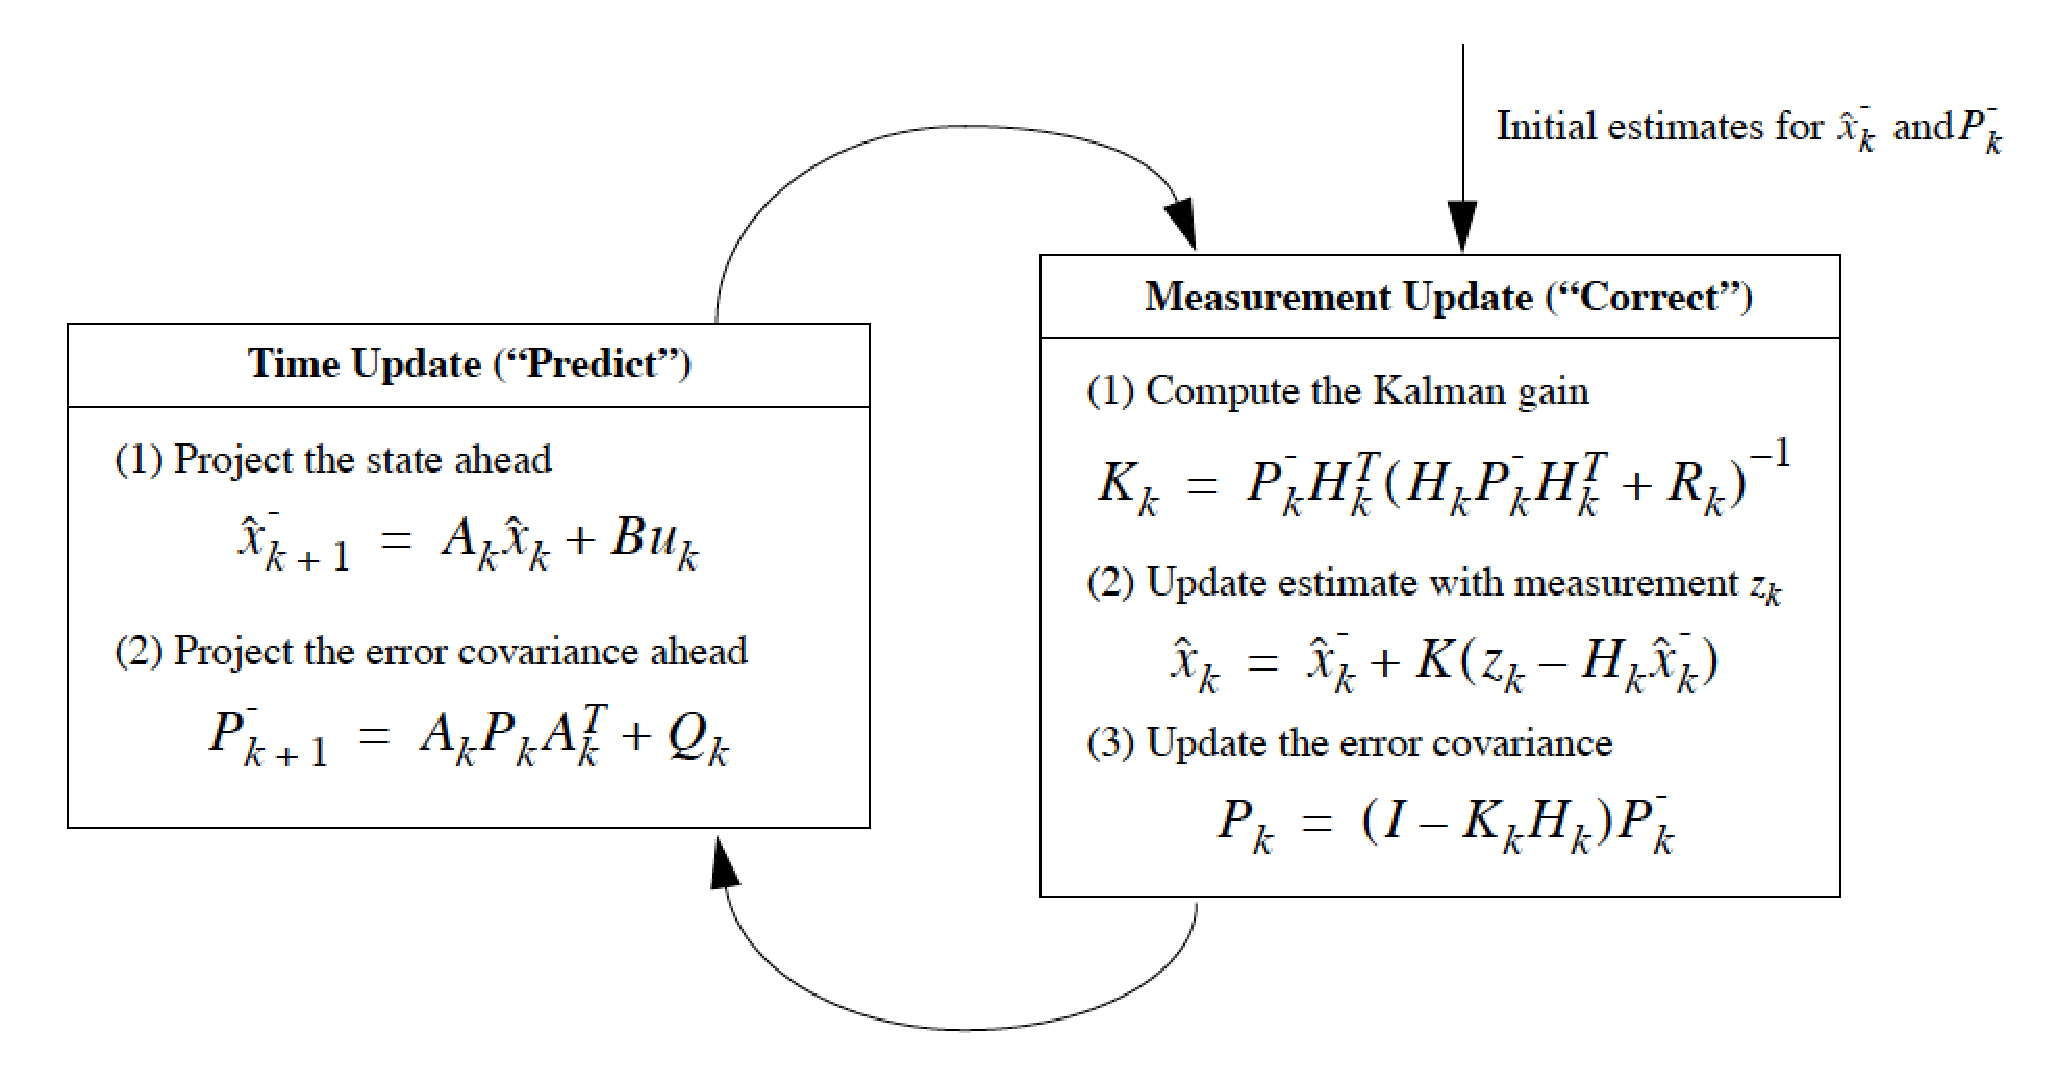
\includegraphics[width=10cm]{pictures/equation_kalman.eps}
\caption{The prediction and the correction step with their corresponding equations. }
\label{equation_kalman}
\end{center}
\end{figure} 
For a fine tuning of the filter often the measurement error covariance matrix $R_k$ and process noise $Q_k$ can be used. $R_k$ tells us how accurate the sensors and therefore the measurements are. This can be estimated in a first round with some static sensor test or can be found in the data sheets of the sensors. The matrix $Q_k$ describes how correct the propagation model described by the matrix $A_k$ is. In this sense as higher the values and therefore the noise of $R_k$ and $Q_k$ as less influence do the measurements or the propagation model respectively have on the estimated state. Having a diagonal matrix with constant values over time, does not represent the reality, but brings it to a form which is fast stable and easier tunable[..pap..]. 

\subsection*{Extended Kalman Filter (EKF)}\label{ekf}
In reality the process to estimate the new state and the measurement relationship to the process is non-linear.
\begin{equation}
x_{k+1}=f(x_k,u_k,w)
z_k=h(x_k,v_k)
\end{equation}
One of the solution to overcome this problem is the Extended Kalman Filter shortly EKF. The EKF is linearizing the this functions with a first order Taylor-Series around the current state. This can be summerized with the following equation:
\begin{equation}
x_{k+1}\approx \hat{x}_{k+1}+A(x_k-\hat{x}_k)+w\\
z_k\approx \hat{z}_k+H(x_k-\hat{x}_k) +v 
\end{equation}
Where $A$ and $H$ are the Jacobian matrix of the function $f$ and $h$.
\begin{equation}
A_{i,j}=\frac{\partial f_{i}}{\partial x_j}(\hat{x}_k,u_k,9)\\
H_{i,j}=\frac{\partial h_{i}}{\partial x_j}(\hat{x}_k,u_k,9)
\end{equation}
This brings us to the summarized equations of the EKF in figure \ref{equation_ekf}.
\begin{figure}[h]
\begin{center}
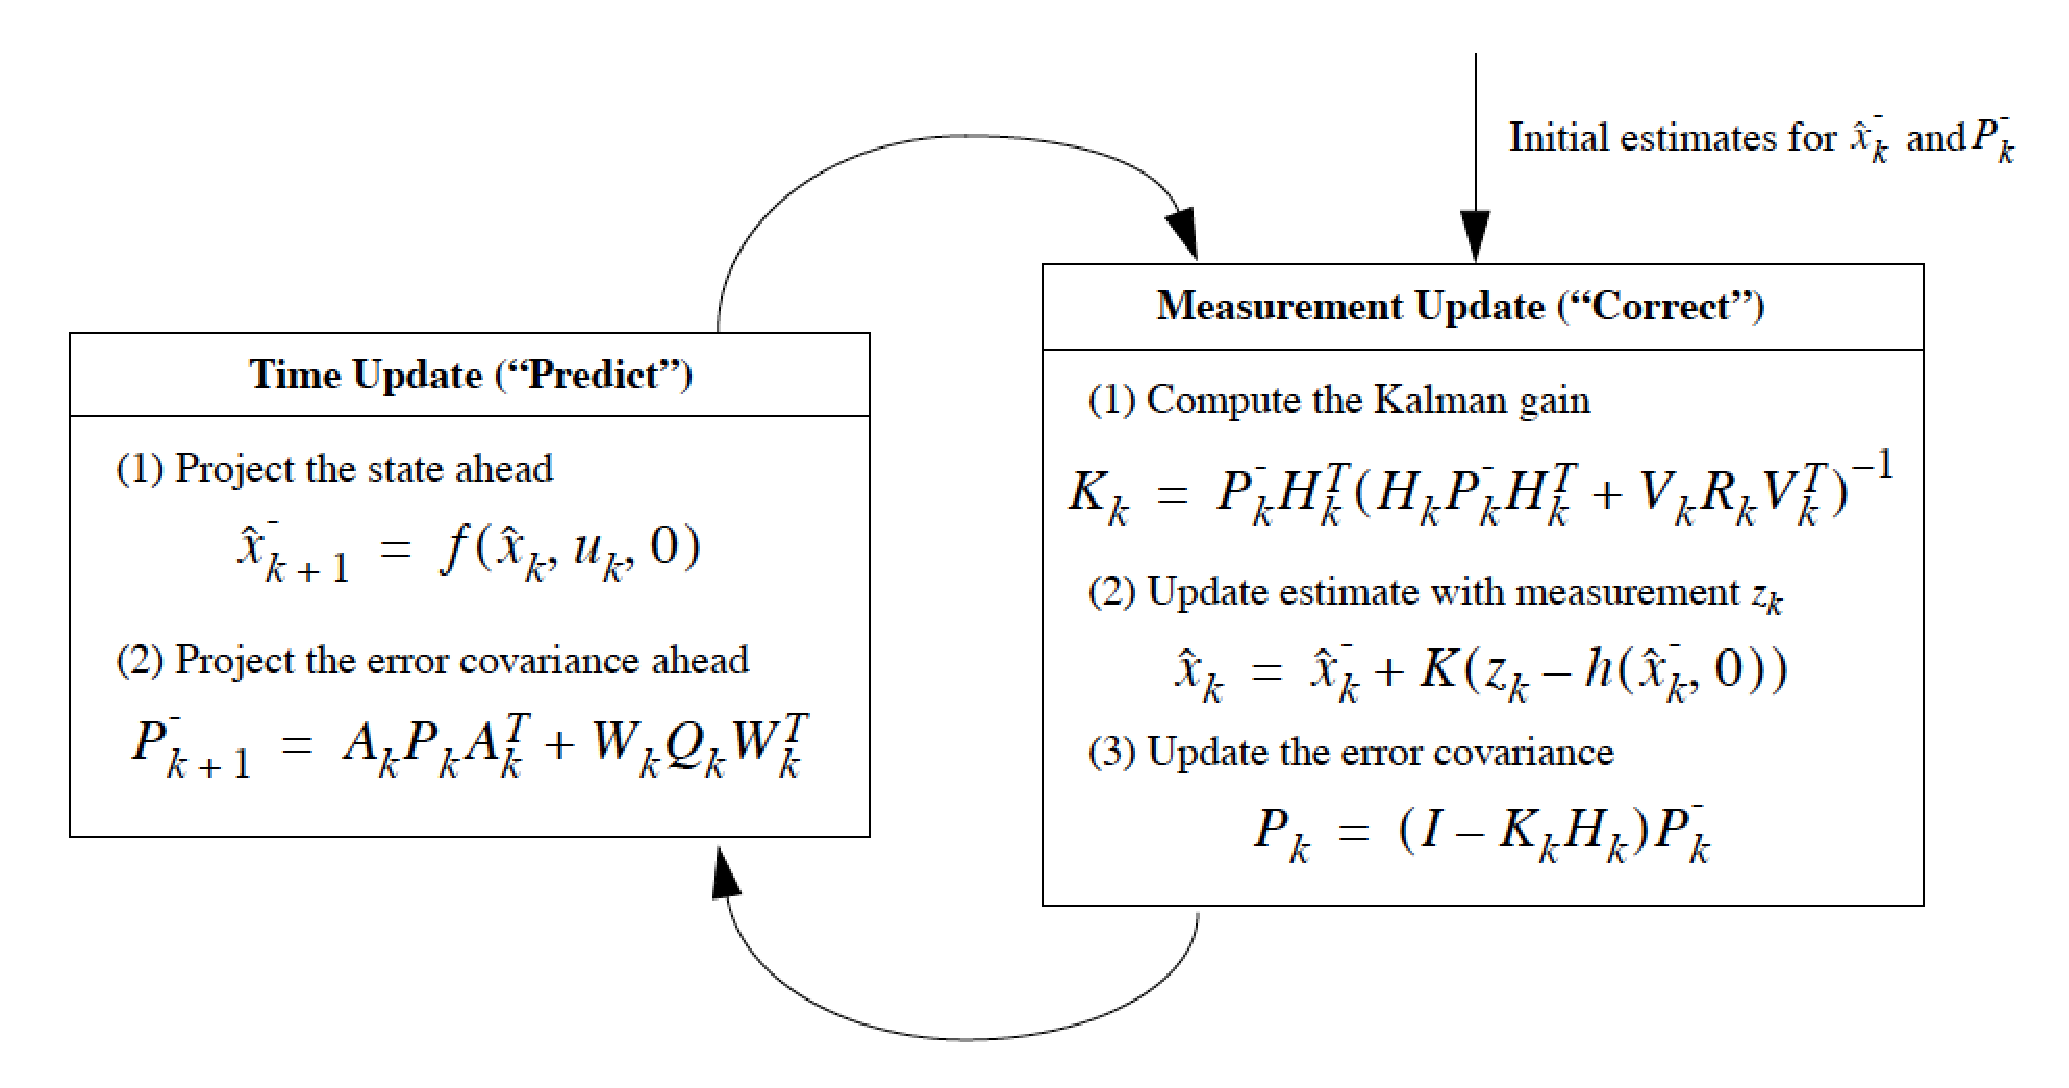
\includegraphics[width=10cm]{pictures/equation_ekf.eps}
\caption{The prediction and correction step of the EKF with their corresponding equations. }
\label{equation_ekf}
\end{center}
\end{figure}
\section{Algorithm for State Estimation}
In this chapter will be explained, how the structure of the algorithm looks like. As mentioned before is the goal to get a as precise as possible estimation of the state with the EKF. The Algorithm has to solve some main problems. First the physical relations between the state $x_{k}$ and the state $x_{k+1}$ has to be defined and summarized in a propagation model. This is needed to calculate the a priori state estimation like described in chapter \ref{math_kalman}. Since this is one of the main points deciding on how accurate the estimation is, is it described in chapter \ref{state_estimation}. A second key role plays the measurement estimation which corrects the a priori state estimation and calculates the a posteriori state estimation. A third question which will be treated in the current section is how the algorithm has to behave in the case of no sensor data is used or of not all sensors provide an output with the same frequency. In the last paragraph is explained on how the error covariances are chosen. Although they were found more with a trial and error method, than based on test, values and known relationships.
The filter is implemented in MATLAB.

\subsection*{States and Measurements}
The state vector with the dimension of 12looks as follows. The measurements used from the IMU is the position (pos) and the velocity (vel) of the GPS, the acceleration (acc) from the accelerometer and the rate of turn (gyro) from the gyroscope and the orientation (mag) from the magnetometer. Each of them in all three dimensions give us the measurement vector z with a dimension of 15.

\begin{equation}
 %x=
 %\begin{pmatrix}
  %pos&x \\
  %pos&y \\
  %pos&z \\
  %vel&x \\
  %vel&y \\
  %vel&z \\
  %acc&x \\
  %acc&y \\
  %acc&z \\
  %gyro&x \\
  %gyro&y \\
  %gyro&z \\
  %mag&x \\
  %mag&y \\
  %mag&z \\
 %\end{pmatrix}
 z= \begin{bmatrix}
  pos\;x \\
  pos\;y \\
  pos\;z \\
  vel\;x \\
  vel\;y \\
  vel\;z \\
  acc\;x \\
  acc\;y \\
  acc\;z \\
  gyro\;x \\
  gyro\;y \\
  gyro\;z \\
  mag\;x \\
  mag\;y \\
  mag\;z
 \end{bmatrix}
\end{equation}

\subsection*{Orientation}
The filter has to handle two different coordinates frames. One is the inertial frame and the other the body frame. The inertial frame is the global frame. The position and the velocity both provided by the GPS are in the inertial frame. The body frame is a coordinate system on the kite. The sensor measurements except the GPS are in the body frame.
The euler angles describe how the inertial frame has to be rotated to bring into the body frame. With other words, the euler angles tell us the orientation of the body frame/ kite. With the direct cosine matrix ($DCM$) we can transform a vector from the inertial frame into the body frame and vise versa. For example can the accelerometer data which is given in body frame coordinates be transformed into the inertial frame, where the propagation of the states is calculated.[..angus..]

\subsection*{Structure of the Algorithm}
In \ref{structure_algo} the schematic of the algorithm is shown. Each of the blocks will now successive explained.
\begin{figure}
\begin{center}
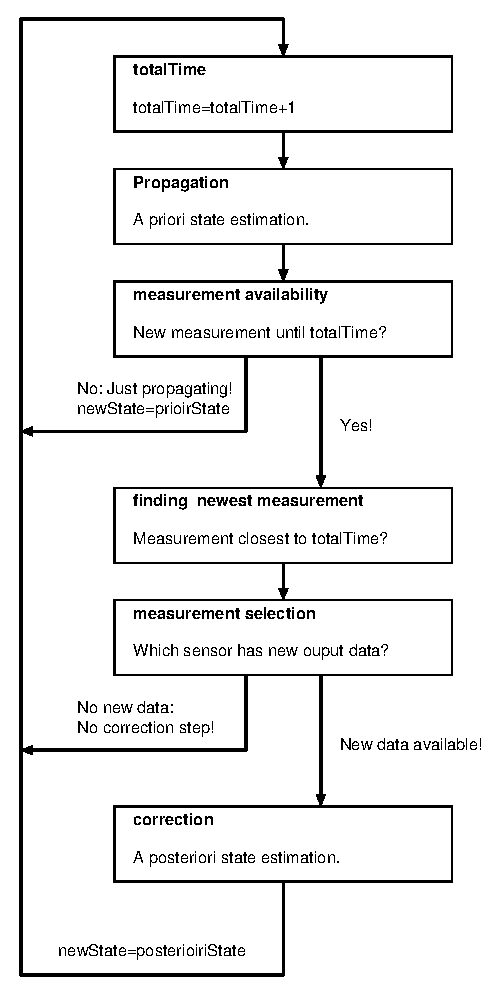
\includegraphics[width=8 cm]{pictures/structure_algo_1.eps}
\caption{The graphical represenetation of the algorithm's structure.}
\label{structure_algo}
\end{center}
\end{figure}

\item[Block 1, totalTime:]
The filter estimates with constant rate the state of the system. This rate is independent on any output rate of the sensors. In the first block the time at which the state is estimated is set. It is the old time totalTime added with the constant time step t.

\item[Block 2, Propagation:]
During the second block the a priori state of the system is estimated with the help of the physical model. How and why the physical model is defined is explained in chapter \ref{state_estimation}. After this step the vector $x_{est}$ is up to date.

\item[Block 3, measurement availability:]
If there is no new measurement until the time of the a priori estimated state, the correction step is not executed. This allows the algorithm to run the ekf with a higher rate, then the IMU provide data. To summarize: If we have no new data from the sensors the system just keeps propagating based on the physical model.

\item[Block 4, finding the closest measurement:]
In this block it is searched for the closest measurement to the time of the a priori estimated state in block 2. If until the time of the estimation several sensor values are available only the newest and therefore most accurate value is taken for the correction.

\item[Block 5, measurement selection:]
Mostly not all sensors of an IMU provide an output with the same rate. Here it is tested, weather we have a new sensor value or is it still the one of the previous estimation. The correction step in block 5 is only for the new data executed. The other one still just propagate.

\item[Block 6, correction:]
As last step the correction of the a priori estimation takes place and the posteriori estimation is calculated. How the relationship between the state and the measurements look like is explained in chapter \ref{sensor_estimation}

\subsection*{Error Covariance}
For the measurement error covariance the noise of the different sensors are taken from the data sheets. But  they were manually scaled according to have more accurate and stable filter. For the propagation model the covariance was estimated on how accurate the equations are. But also in this case were they manually adjusted afterwards. For an easier handling only the diagonal elements have a value. The off diagonal values are all zero.
\subsection*{Jacobian Matrix}
In chapter \ref{ekf} the matrixes H and A were derived. Since the physical model and relations between state and the measurements are non linear, H and A are the Jacobian matrixes of the functions $f$ and $h$. For having an accurate as possible solution the Jacobian was in a first version calculated analytically with symbolic toolbox from MathWorks. The Jacobian matrix then has to be evaluated in every iteration step. Simulating 0.01 seconds took the filter much longer than 10 minutes. It was then decided to rewrite the algorithm calculating the Jacobian matrixes numerical. The function ekf.m [..ekfwebsite..]from MathWorks was restructured to match the requirements of this algorithm. It uses a complex step differentiation to calculate the derivatives of the function f and h [..papCompDiff..]. 
\section{State Estimation Model}\label{state_estimation}
\section{Sensor Estimation Model}\label{sensor_estimation}
An illustration of the relation between the position and velocity in $(y,x,z)$ or $(dx,dy,dz)$ and the two angles …. is shown in (...figure...). With this sketch and the fact that the velocity is the derivative of the position we get to the equations: 
The centripetal acceleration can be calculated by the formula:
We then have the additional acceleration of the earth gravitation. The earth gravitation is in the inertial frame only in z direction and has to be transformed with the $DCM_{bi}$ from the inertial in the body frame. The magnetic field is given in the inertial frame in Zurich by :...... . By transforming that into the body frame again with the help of the $DCM_{bi}$, the expected measurement from the magnetometer is calculated. Because the position of the senors is not at the center of mass of the pendulum, an additional displacement vector has to be added to the position (compare figure \ref{displacement}). With transforming the distance between the center of mass and the sensor into the inertial frame, the position is adjusted. The displacement gives an additional velocity which is the crossproduct of the rate of rotation and the displacement from the center of mass.
\begin{figure}[h]
\begin{center}
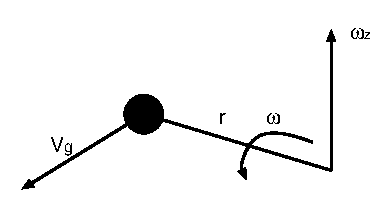
\includegraphics[width=8 cm]{pictures/displacement_1.eps}
\caption{The black dot represents the sensor, while r is the distance between the center of mass of the pendulum and the sensor.}
\label{displacement}
\end{center}
\end{figure}

